\documentclass[8pt,aspectratio=169]{beamer}
\usetheme{Madrid}
\usepackage{graphicx}
\usepackage{booktabs}
\usepackage{adjustbox}
\usepackage{multicol}
\usepackage{amsmath}
\usepackage{amssymb}
\usepackage{tikz}
\usepackage{hyperref}
\usepackage{algorithm}
\usepackage{algorithmic}
\usepackage{colortbl}
\usepackage{pgfplots}
\pgfplotsset{compat=1.18}

% TikZ libraries for comics, diagrams, stakeholder maps
\usetikzlibrary{arrows.meta,positioning,shapes.callouts,shapes.geometric,decorations.pathreplacing}

% Color definitions
\definecolor{mlblue}{RGB}{0,102,204}
\definecolor{mlpurple}{RGB}{51,51,178}
\definecolor{mllavender}{RGB}{173,173,224}
\definecolor{mllavender2}{RGB}{193,193,232}
\definecolor{mllavender3}{RGB}{204,204,235}
\definecolor{mllavender4}{RGB}{214,214,239}
\definecolor{mlorange}{RGB}{255, 127, 14}
\definecolor{mlgreen}{RGB}{44, 160, 44}
\definecolor{mlred}{RGB}{214, 39, 40}
\definecolor{mlgray}{RGB}{127, 127, 127}
\definecolor{lightgray}{RGB}{240, 240, 240}
\definecolor{midgray}{RGB}{180, 180, 180}

% NEW COLORS for mini-lecture
\definecolor{dfteal}{RGB}{0,128,128}
\definecolor{dfred}{RGB}{180,30,30}

% Backward compatibility
\colorlet{MLPurple}{mlpurple}
\colorlet{MLBlue}{mlblue}
\colorlet{MLOrange}{mlorange}
\colorlet{MLGreen}{mlgreen}
\colorlet{MLRed}{mlred}
\colorlet{MLLavender}{mllavender}
\colorlet{MLGray}{mlgray}

% Theme colors (exact Madrid settings)
\setbeamercolor{palette primary}{bg=mllavender3,fg=mlpurple}
\setbeamercolor{palette secondary}{bg=mllavender2,fg=mlpurple}
\setbeamercolor{palette tertiary}{bg=mllavender,fg=white}
\setbeamercolor{palette quaternary}{bg=mlpurple,fg=white}
\setbeamercolor{structure}{fg=mlpurple}
\setbeamercolor{section in toc}{fg=mlpurple}
\setbeamercolor{subsection in toc}{fg=mlblue}
\setbeamercolor{title}{fg=mlpurple}
\setbeamercolor{frametitle}{fg=mlpurple,bg=mllavender3}
\setbeamercolor{block title}{bg=mllavender2,fg=mlpurple}
\setbeamercolor{block body}{bg=mllavender4,fg=black}
\setbeamertemplate{navigation symbols}{}
\setbeamertemplate{itemize items}[circle]
\setbeamertemplate{enumerate items}[default]
\setbeamersize{text margin left=5mm,text margin right=5mm}

% Footer
\setbeamertemplate{footline}{
  \leavevmode%
  \hbox{%
    \begin{beamercolorbox}[wd=.333333\paperwidth,ht=2.25ex,dp=1ex,center]{author in head/foot}%
      \usebeamerfont{author in head/foot}Methods and Algorithms
    \end{beamercolorbox}%
    \begin{beamercolorbox}[wd=.333333\paperwidth,ht=2.25ex,dp=1ex,center]{title in head/foot}%
      \usebeamerfont{title in head/foot}MSc Data Science
    \end{beamercolorbox}%
    \begin{beamercolorbox}[wd=.333333\paperwidth,ht=2.25ex,dp=1ex,right]{date in head/foot}%
      \usebeamerfont{date in head/foot}\insertframenumber{} / \inserttotalframenumber\hspace*{2ex}
    \end{beamercolorbox}}%
  \vskip0pt%
}

\newcommand{\bottomnote}[1]{%
\vfill
\vspace{-2mm}
\textcolor{mllavender2}{\rule{\textwidth}{0.4pt}}
\vspace{1mm}
\footnotesize
\textbf{#1}
}

\newenvironment{compactlist}{%
  \begin{itemize}%
    \setlength{\itemsep}{2pt}%
    \setlength{\parskip}{0pt}%
    \setlength{\parsep}{0pt}%
}{%
  \end{itemize}%
}

\newcommand{\highlight}[1]{\textcolor{mlorange}{\textbf{#1}}}
\newcommand{\mathbold}[1]{\boldsymbol{#1}}

% =====================================================
\title[RL Full Lecture]{Reinforcement Learning}
\subtitle{Learning to Act from Rewards}
\author{Methods \& Algorithms}
\date{MSc Data Science -- Spring 2026}

\begin{document}

% =====================================================
% INTRO ZONE (slides 1-5, NO formulas)
% =====================================================

% --- Slide 1: Title ---
\begin{frame}
\titlepage
\end{frame}

% --- Slide 2: Opening Comic ---
\begin{frame}{Can a Machine Learn to Trade Stocks by Trial and Error?}
\centering
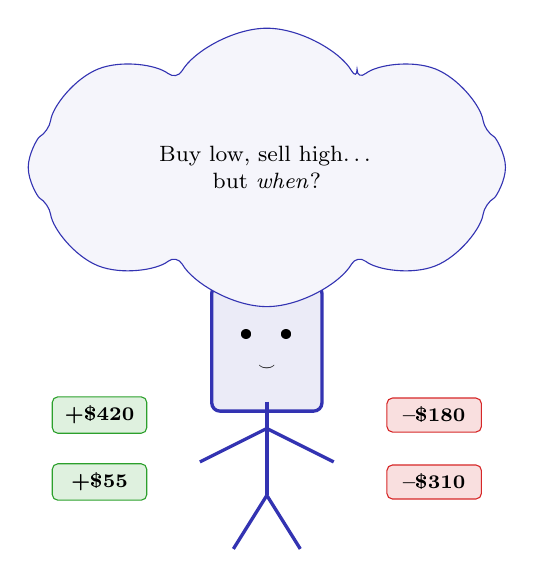
\begin{tikzpicture}[scale=0.85]
  % Robot trader
  \node[draw=mlpurple, fill=mlpurple!10, rounded corners=3pt,
        minimum width=1.4cm, minimum height=1.6cm, line width=1.2pt] (head) at (0,2.5) {};
  \node at (-0.3,2.7) {\small\textbullet};
  \node at (0.3,2.7) {\small\textbullet};
  \node at (0,2.2) {\tiny $\smile$};
  % Antenna
  \draw[mlpurple, line width=1pt] (0,3.3) -- (0,3.8);
  \fill[mlpurple] (0,3.8) circle (2pt);
  % Body
  \draw[mlpurple, line width=1.2pt] (0,1.7) -- (0,0.3);
  \draw[mlpurple, line width=1.2pt] (0,1.3) -- (-1,0.8);
  \draw[mlpurple, line width=1.2pt] (0,1.3) -- (1,0.8);
  \draw[mlpurple, line width=1.2pt] (0,0.3) -- (-0.5,-0.5);
  \draw[mlpurple, line width=1.2pt] (0,0.3) -- (0.5,-0.5);
  % Screens
  \node[draw=mlgreen, fill=mlgreen!15, rounded corners=2pt, font=\scriptsize,
        minimum width=1.2cm] at (-2.5,1.5) {\textbf{+\$420}};
  \node[draw=mlred, fill=mlred!15, rounded corners=2pt, font=\scriptsize,
        minimum width=1.2cm] at (2.5,1.5) {\textbf{--\$180}};
  \node[draw=mlgreen, fill=mlgreen!15, rounded corners=2pt, font=\scriptsize,
        minimum width=1.2cm] at (-2.5,0.5) {\textbf{+\$55}};
  \node[draw=mlred, fill=mlred!15, rounded corners=2pt, font=\scriptsize,
        minimum width=1.2cm] at (2.5,0.5) {\textbf{--\$310}};
  % Thought bubble
  \node[draw=mlpurple, fill=mlpurple!5, rounded corners=4pt, cloud, cloud puffs=8,
        cloud puff arc=120, aspect=2.5, text width=4cm, align=center,
        font=\footnotesize] at (0,5.2) {Buy low, sell high\ldots\\ but \textit{when}?};
\end{tikzpicture}

\bottomnote{RL agents learn from outcomes, not from labeled examples.}
\end{frame}

% --- Slide 3: Learning Objectives ---
\begin{frame}{Learning Objectives}
After this lecture, you will be able to:
\begin{enumerate}
  \item \textbf{Formalize} sequential decisions as Markov Decision Processes
  \item \textbf{Derive} the Bellman equation and implement Q-learning
  \item \textbf{Analyze} exploration-exploitation trade-offs using epsilon-greedy
  \item \textbf{Apply} RL to algorithmic trading and portfolio management
\end{enumerate}

\bottomnote{LOs at Bloom's levels 4--5: formalize, derive, analyze, apply.}
\end{frame}

% --- Slide 4: What Is RL? ---
\begin{frame}{What Is Reinforcement Learning?}
\begin{columns}[T]
\begin{column}{0.52\textwidth}
An \highlight{agent} learns to make decisions by interacting with an
\textbf{environment} and receiving \textbf{rewards}.

\vspace{4pt}
\begin{compactlist}
  \item Not supervised: no labeled ``correct actions''
  \item Not unsupervised: there is a goal (maximize reward)
  \item Learning by \textbf{trial and error}
\end{compactlist}
\end{column}
\begin{column}{0.45\textwidth}
\begin{block}{Key Terms}
\begin{compactlist}
  \item \textbf{Agent}: the learner / decision-maker
  \item \textbf{Environment}: the world it acts in
  \item \textbf{State}: current situation
  \item \textbf{Action}: what the agent does
  \item \textbf{Reward}: feedback signal
  \item \textbf{Policy}: action selection strategy
\end{compactlist}
\end{block}
\end{column}
\end{columns}

\bottomnote{RL sits between supervised and unsupervised learning: it has a goal but no labels.}
\end{frame}

% --- Slide 5: Why Not Supervised? ---
\begin{frame}{Why Not Just Use Supervised Learning?}
\begin{columns}[T]
\begin{column}{0.48\textwidth}
\textbf{Supervised Learning}
\begin{compactlist}
  \item Needs labeled data $(x, y)$
  \item ``What is the correct action?'' requires a label
  \item Assumes i.i.d.\ samples
\end{compactlist}
\end{column}
\begin{column}{0.48\textwidth}
\textbf{Reinforcement Learning}
\begin{compactlist}
  \item Learns from outcomes (reward signals)
  \item No one tells you the ``right'' trade
  \item Delayed rewards: today's trade affects tomorrow
\end{compactlist}
\end{column}
\end{columns}

\bottomnote{In trading, you only know if a decision was good after the market moves.}
\end{frame}

% =====================================================
% CORE -- METHOD (slides 6-14)
% =====================================================

% --- Slide 6: Agent-Environment Loop (chart) ---
\begin{frame}{The Agent-Environment Loop}
\centering

\includegraphics[width=0.65\textwidth]{03_rl_loop/chart.pdf}

\bottomnote{State $\rightarrow$ Action $\rightarrow$ Reward $\rightarrow$ Next State $\rightarrow$ repeat.}
\end{frame}

% --- Slide 7: MDP ---
\begin{frame}{Markov Decision Process (MDP)}
\begin{block}{Definition}
An MDP is a tuple $(S, A, P, R, \gamma)$:
\begin{compactlist}
  \item $S$: set of states \quad $A$: set of actions
  \item $P(s' \mid s, a)$: transition probability
  \item $R(s, a)$: reward function \quad $\gamma \in [0,1]$: discount factor
\end{compactlist}
\end{block}

\vspace{4pt}
\textbf{Markov property}: the future depends only on the current state, not the history.
\[
  P(S_{t+1} \mid S_t, A_t) = P(S_{t+1} \mid S_0, A_0, \ldots, S_t, A_t)
\]

\bottomnote{The MDP formalism is the mathematical foundation of all RL algorithms.}
\end{frame}

% --- Slide 8: Return and Value Functions ---
\begin{frame}{The Return and Value Functions}
\textbf{Return} (discounted cumulative reward):
\[
  G_t = \sum_{k=0}^{\infty} \gamma^k R_{t+k+1}
\]

\textbf{State-value function} (how good is state $s$?):
\[
  V^\pi(s) = \mathbb{E}_\pi\bigl[G_t \mid S_t = s\bigr]
\]

\textbf{Action-value function} (how good is action $a$ in state $s$?):
\[
  Q^\pi(s, a) = \mathbb{E}_\pi\bigl[G_t \mid S_t = s,\, A_t = a\bigr]
\]

\bottomnote{$\gamma$ close to 1: far-sighted agent. $\gamma$ close to 0: myopic agent.}
\end{frame}

% --- Slide 9: Bellman Equation ---
\begin{frame}{The Bellman Equation}
The optimal action-value satisfies a \highlight{recursive} relationship:
\[
  Q^*(s,a) = R(s,a) + \gamma \sum_{s'} P(s' \mid s,a)\,\max_{a'} Q^*(s',a')
\]
\scriptsize\textcolor{mlgray}{This expands the $\mathbb{E}[\cdot]$ form from the overview by substituting transition probabilities $P(s'|s,a)$.}

\normalsize
\textbf{Worked example} ($\gamma = 0.9$, deterministic transitions):

\begin{compactlist}
  \item State A $\xrightarrow{\text{right}}$ State B, reward $= +1$
  \item State B $\xrightarrow{\text{right}}$ State C (terminal, $Q=0$ by definition), reward $= +10$
  \item $Q(B, \text{right}) = 10 + 0.9 \times 0 = 10$
  \item $Q(A, \text{right}) = 1 + 0.9 \times 10 = 10$
\end{compactlist}

\bottomnote{The Bellman equation decomposes value into immediate reward + discounted future.}
\end{frame}

% --- Slide 10: Q-Learning (chart) ---
\begin{frame}{Q-Learning: Model-Free Temporal Difference}
\begin{columns}[T]
\begin{column}{0.48\textwidth}
\textbf{Update rule}:
\[
  Q(s,a) \leftarrow Q(s,a) + \alpha\bigl[R + \gamma\max_{a'}Q(s',a') - Q(s,a)\bigr]
\]
\begin{compactlist}
  \item $\alpha$: learning rate
  \item No transition model $P$ needed!
  \item Converges to $Q^*$ with sufficient exploration
\end{compactlist}
\end{column}
\begin{column}{0.48\textwidth}

\includegraphics[width=\textwidth]{04_q_learning_grid/chart.pdf}
\end{column}
\end{columns}

\bottomnote{Q-learning is off-policy: it learns the optimal Q regardless of the behavior policy.}
\end{frame}

% --- Slide 11: Exploration vs Exploitation ---
\begin{frame}{Exploration vs Exploitation}
\begin{columns}[T]
\begin{column}{0.48\textwidth}
\textbf{The Dilemma}
\begin{compactlist}
  \item \textbf{Exploit}: choose the best known action
  \item \textbf{Explore}: try a random action to discover more
  \item Too much exploitation $\rightarrow$ stuck at local optimum
  \item Too much exploration $\rightarrow$ never converges
\end{compactlist}
\end{column}
\begin{column}{0.48\textwidth}
\textbf{Epsilon-Greedy Policy}
\begin{compactlist}
  \item With probability $\varepsilon$: random action
  \item With probability $1-\varepsilon$: greedy action
  \item \textbf{Decaying $\varepsilon$}: explore early, exploit later
\end{compactlist}
\end{column}
\end{columns}

\bottomnote{Balancing exploration and exploitation is a fundamental challenge in RL.}
\end{frame}

% --- Slide 12: Reward Curves (chart) ---
\begin{frame}{Watching the Agent Learn}
\begin{columns}[T]
\begin{column}{0.40\textwidth}
\begin{compactlist}
  \item Early episodes: near-random, low reward
  \item Mid training: discovers good paths
  \item Late training: converges to optimal policy
\end{compactlist}
\end{column}
\begin{column}{0.55\textwidth}

\includegraphics[width=\textwidth]{05_reward_curves/chart.pdf}
\end{column}
\end{columns}

\bottomnote{The learning curve shows cumulative reward increasing as the agent improves.}
\end{frame}

% --- Slide 13: Policy Visualization (chart) ---
\begin{frame}{Visualizing the Learned Policy}
\centering

\includegraphics[width=0.65\textwidth]{06_policy_viz/chart.pdf}

\bottomnote{Arrows show the optimal action in each state -- the agent has learned to navigate.}
\end{frame}

% --- Slide 14: DQN (chart) ---
\begin{frame}{Deep Q-Networks (DQN)}
\begin{columns}[T]
\begin{column}{0.45\textwidth}
\begin{compactlist}
  \item Replace Q-table with a \highlight{neural network}
  \item Input: state $\rightarrow$ Output: $Q(s,a)$ for all $a$
  \item \textbf{Experience replay}: store and resample transitions
  \item \textbf{Target network}: stabilize training
\end{compactlist}
\vspace{4pt}
Scales to continuous or very large state spaces.
\end{column}
\begin{column}{0.52\textwidth}

\includegraphics[width=\textwidth]{09_dqn_architecture/chart.pdf}
\end{column}
\end{columns}

\bottomnote{DQN (Mnih et al., 2015) enabled RL to play Atari games from raw pixels.}
\end{frame}

% =====================================================
% CORE -- SOLUTION (slides 15-19)
% =====================================================

% --- Slide 15: Trading as MDP ---
\begin{frame}{Algorithmic Trading as an MDP}
\begin{columns}[T]
\begin{column}{0.48\textwidth}
\textbf{MDP Formulation}
\begin{compactlist}
  \item \textbf{State}: (price, position, time)
  \item \textbf{Actions}: buy, sell, hold
  \item \textbf{Reward}: realized P\&L per step
\end{compactlist}
\end{column}
\begin{column}{0.48\textwidth}
\textbf{Why RL Fits}
\begin{compactlist}
  \item Sequential decisions over time
  \item Delayed reward (hold for days)
  \item No ``correct label'' for each action
\end{compactlist}
\end{column}
\end{columns}

\bottomnote{The trading agent learns when to enter and exit positions to maximize returns.}
\end{frame}

% --- Slide 16: Portfolio Optimization ---
\begin{frame}{Portfolio Optimization with RL}
\begin{columns}[T]
\begin{column}{0.48\textwidth}
\textbf{Setup}
\begin{compactlist}
  \item \textbf{State}: portfolio weights + market features
  \item \textbf{Action}: rebalance weights
  \item \textbf{Reward}: risk-adjusted return (Sharpe ratio)
\end{compactlist}
\end{column}
\begin{column}{0.48\textwidth}
\textbf{Advantages}
\begin{compactlist}
  \item Handles transaction costs naturally
  \item Adapts to changing market regimes
  \item Optimizes multi-period objectives
\end{compactlist}
\end{column}
\end{columns}

\bottomnote{RL-based portfolio management optimizes the Sharpe ratio while accounting for costs.}
\end{frame}

% --- Slide 17: Optimal Execution ---
\begin{frame}{Optimal Execution: Minimizing Market Impact}
\textbf{Problem}: Execute a large order without moving the market.

\begin{enumerate}
  \item Split the order into smaller slices over time
  \item \textbf{State}: remaining shares, time left, market volatility
  \item \textbf{Action}: how many shares to trade now
  \item \textbf{Reward}: $-$slippage cost (minimize market impact)
\end{enumerate}

\vspace{4pt}
The RL agent learns to trade more aggressively in calm markets
and slow down during volatile periods.

\bottomnote{Optimal execution is one of the most commercially successful RL applications in finance.}
\end{frame}

% --- Slide 18: Reward Engineering ---
\begin{frame}{Reward Engineering: The Hardest Part of RL}
\begin{columns}[T]
\begin{column}{0.48\textwidth}
\textbf{\textcolor{mlred}{Bad Reward Design}}
\begin{compactlist}
  \item Maximize raw return $\rightarrow$ extreme leverage
  \item Maximize win rate $\rightarrow$ tiny gains, huge losses
  \item No drawdown penalty $\rightarrow$ reckless risk
\end{compactlist}
\end{column}
\begin{column}{0.48\textwidth}
\textbf{\textcolor{mlgreen}{Better Reward Design}}
\begin{compactlist}
  \item Sharpe ratio: return / volatility
  \item Drawdown penalty: punish large losses
  \item Risk-adjusted P\&L with position limits
\end{compactlist}
\end{column}
\end{columns}

\vspace{4pt}
\centering
\textit{``The reward function IS your specification of the problem.''}

\bottomnote{Misaligned rewards produce agents that technically optimize but behave badly.}
\end{frame}

% --- Slide 19: RL Challenges ---
\begin{frame}{RL Challenges in Finance}
\begin{columns}[T]
\begin{column}{0.48\textwidth}
\textbf{Technical Challenges}
\begin{compactlist}
  \item \textbf{Non-stationarity}: markets change over time
  \item \textbf{Partial observability}: you cannot see everything
  \item \textbf{Sample efficiency}: live trading data is expensive
\end{compactlist}
\end{column}
\begin{column}{0.48\textwidth}
\textbf{Practical Challenges}
\begin{compactlist}
  \item \textbf{Sim-to-real gap}: backtests $\neq$ live markets
  \item \textbf{Regime changes}: bull $\rightarrow$ bear invalidates policy
  \item \textbf{Regulatory}: explain decisions to compliance
\end{compactlist}
\end{column}
\end{columns}

\bottomnote{These challenges are why RL in finance remains an active research frontier.}
\end{frame}

% =====================================================
% CLOSING (slides 20-25)
% =====================================================

% --- Slide 20: When to Use ---
\begin{frame}{When to Use RL -- and When Not To}
\begin{columns}[T]
\begin{column}{0.48\textwidth}
\textbf{\textcolor{mlgreen}{Pros}}
\begin{compactlist}
  \item Handles sequential decision problems
  \item No labeled data required
  \item Adapts to changing environments
\end{compactlist}
\end{column}
\begin{column}{0.48\textwidth}
\textbf{\textcolor{mlred}{Cons}}
\begin{compactlist}
  \item Slow training, high sample cost
  \item Reward design is hard to get right
  \item Sim-to-real gap in finance
  \item Difficult to interpret and debug
\end{compactlist}
\end{column}
\end{columns}

\bottomnote{Use RL when decisions are sequential and delayed -- not for one-shot predictions.}
\end{frame}

% --- Slide 21: Comparison Table ---
\begin{frame}{RL vs Supervised Learning vs Optimization}
\small
\begin{tabular}{p{2.5cm}p{3cm}p{3cm}p{3cm}}
\toprule
& \textbf{Supervised} & \textbf{RL} & \textbf{Optimization} \\
\midrule
Data & Labeled $(x,y)$ & Reward signal & Objective function \\
Sequential & No & Yes & Sometimes \\
Adapts & Retrain needed & Online learning & Re-solve \\
Interpretable & Model-dependent & Low & High \\
Training time & Fast & Slow & Medium \\
\bottomrule
\end{tabular}

\bottomnote{Each paradigm has its sweet spot -- RL shines for sequential, adaptive problems.}
\end{frame}

% --- Slide 22: Hands-on ---
\begin{frame}[fragile]{Hands-on: Train a Q-Learning Agent}
\small
\begin{verbatim}
import numpy as np
# 5x5 gridworld: start (0,0), goal (4,4)
Q = np.zeros((25, 4))  # 25 states, 4 actions
alpha, gamma, epsilon = 0.1, 0.99, 0.1

for episode in range(500):
    s = 0  # start state
    while s != 24:  # goal state
        if np.random.rand() < epsilon:
            a = np.random.randint(4)
        else:
            a = np.argmax(Q[s])
        s_next, r = step(s, a)  # environment step
        Q[s,a] += alpha * (r + gamma*np.max(Q[s_next]) - Q[s,a])
        s = s_next
\end{verbatim}
\vspace{2pt}
\small Full notebook: \texttt{L06\_rl.ipynb}

\bottomnote{Try the notebook to train your own gridworld agent and visualize the policy.}
\end{frame}

% --- Slide 23: Key Takeaways ---
\begin{frame}{Key Takeaways}
\begin{columns}[T]
\begin{column}{0.48\textwidth}
\textbf{Concepts}
\begin{compactlist}
  \item MDP formalizes sequential decisions
  \item Bellman equation decomposes value recursively
  \item Q-learning is model-free and off-policy
  \item DQN scales Q-learning to large state spaces
\end{compactlist}
\end{column}
\begin{column}{0.48\textwidth}
\textbf{Practice}
\begin{compactlist}
  \item Start with tabular Q-learning
  \item Reward design matters more than algorithm
  \item Always compare to a simple baseline
  \item Beware overfitting to backtests
\end{compactlist}
\end{column}
\end{columns}

\bottomnote{RL is powerful for sequential decisions but demands careful reward engineering.}
\end{frame}

% --- Slide 24: Course Wrap-Up ---
\begin{frame}{Course Wrap-Up: From Regression to RL}
\begin{compactlist}
  \item \textbf{L01}: Predict (Linear Regression)
  \item \textbf{L02}: Classify (Logistic Regression)
  \item \textbf{L03}: Cluster (KNN \& K-Means)
  \item \textbf{L04}: Ensemble (Random Forests)
  \item \textbf{L05}: Reduce (PCA \& t-SNE)
  \item \textbf{L06}: Represent \& Act (Embeddings \& RL)
\end{compactlist}

\vspace{6pt}
\centering
\textit{Your ML toolbox is complete.}

\bottomnote{Six sessions, six paradigms -- from prediction to decision-making under uncertainty.}
\end{frame}

% --- Slide 25: Closing Comic ---
\begin{frame}{Closing Thought}
\centering
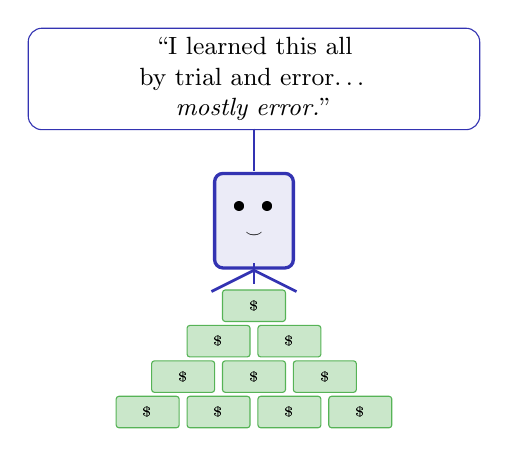
\begin{tikzpicture}[scale=0.9]
  % Pile of money
  \foreach \x/\y in {-1.5/-1.5,-0.5/-1.5,0.5/-1.5,1.5/-1.5,-1/-1,0/-1,1/-1,-0.5/-0.5,0.5/-0.5,0/0} {
    \node[draw=mlgreen!80, fill=mlgreen!25, rounded corners=1pt,
          minimum width=0.8cm, minimum height=0.4cm, font=\tiny] at (\x,\y) {\$};
  }
  % Robot on top
  \node[draw=mlpurple, fill=mlpurple!10, rounded corners=3pt,
        minimum width=1cm, minimum height=1.2cm, line width=1.2pt] (rhead) at (0,1.2) {};
  \node at (-0.2,1.4) {\small\textbullet};
  \node at (0.2,1.4) {\small\textbullet};
  \node at (0,1.0) {\tiny $\smile$};
  \draw[mlpurple, line width=1pt] (0,0.6) -- (0,0.3);
  \draw[mlpurple, line width=1pt] (0,0.5) -- (-0.6,0.2);
  \draw[mlpurple, line width=1pt] (0,0.5) -- (0.6,0.2);
  % Speech bubble
  \node[draw=mlpurple, fill=white, rounded corners=5pt, text width=5.5cm, align=center,
        font=\small] at (0,3.2)
        {``I learned this all by trial and error\ldots\\
        \textit{mostly error.}''};
  \draw[mlpurple, line width=0.8pt] (0,2.5) -- (0,1.9);
\end{tikzpicture}

\bottomnote{Thank you for a great semester! Good luck with your group assignments.}
\end{frame}

\end{document}
